\providecommand{\main}{../..}
\documentclass[\main/main.tex]{subfiles}

\begin{document}

\section{Introduzione ai diodi}

Il diodo è un componente elettronico composto da una giunzione PN.
Il lato P è chiamato "anodo", mentre il lato N è chiamato "catodo".
La presenza delle zone N e P fa sì che gli elettroni liberi e le lacune si muovano, svuotando così la parte centrale del diodo.
A seconda del segno tensione applicata ai capi del diodo, cambia l'estensione della zona centrale svuotata:
\begin{itemize}
  \item Se la tensione è positiva: il diodo lavora in regime di \textbf{polarizzazione diretta} e la zona svuotata si restringe.
  \item Se la tensione è negativa: il diodo lavora in regime di \textbf{polarizzazione inversa} e la zona svuotata si allarga.
\end{itemize}
In un diodo ideale, in regime di polarizzazione diretta nel diodo scorre corrente, mentre in regime di polarizzazione inversa non scorre corrente: in questo caso il diodo (ideale) si comporta infatti come un circuito aperto.

Consideriamo invece un diodo reale.
Le cariche all'interno del diodo si muovono di moto casuale dovuto all'agitazione termica. Questo moto causa una corrente di diffusione non nulla, che può essere calcolata attraverso la \textbf{Legge di Fick}:
\[I_{diff} = A \left[(-q)D_p\frac{\partial p(x)}{\partial x} - (-q)D_n\frac{\partial n(x)}{\partial x} \right]\]
Dove  $D_{p}$ e  $D_{n} $ sono detti "coefficienti di diffusione".

Per calcolare la corrente in regime di polarizzazione \textbf{diretta} si usa la seguente formula:
\[I_D = I_0 \left[e^{\frac{V_D}{V_{Th}}}-1 \right]\]
Dove  $I_0$ è detta "corrente inversa di saturazione" e  $V_{Th} $ è detta "Tensione Termica".
La tensione termica viene calcolata come segue:
\[V_{Th} = \frac{KT}{q}\]
essendo K la costante di Bolzmann. A temperatura ambiente (circa 300 K) essa vale circa 26 mV.

Possiamo descrivere un diodo attraverso tre modelli, con diversi gradi di precisione.

\textbf{Modello 0}:
\begin{itemize}
  \item Inversa: I=0  $\Rightarrow$ Il diodo può essere approssimato a un circuito aperto.
  \item Diretta: I$\rightarrow\infty$  $\Rightarrow$ Il diodo può essere approssimato a un circuito chiuso.
\end{itemize}
\textbf{Modello 1}:
\begin{itemize}
  \item Inversa:  I=0  $\Rightarrow$  Il diodo può essere approssimato a un circuito aperto come nel modello precedente.
  \item Diretta: Il diodo può essere approssimato a un circuito chiuso a cui sia stato aggiunto un generatore che imponga una tensione di 0.7 V.
\end{itemize}
\textbf{Modello 2}:
\begin{itemize}
  \item Inversa: I=0  $\Rightarrow$ Il diodo può essere approssimato a un circuito aperto come nei modelli precedenti.
  \item Diretta: Oltre a collegare in serie al circuito chiuso un generatore di tensione da 0.7 V, aggiungiamo anche una resistenza $R_D$ tale che \[R_D = \frac{V_{Th}}{I_D}\].
\end{itemize}

In un diodo reale può verificarsi l'\textbf{Effetto di Run-Out}: questo fenomeno consiste nel fatto che, a mano a mano che il circuito si scalda, il diodo porta una quantità maggiore di corrente per Effetto Joule, scaldandosi così maggiormente e dissipando maggiore potenza. Per evitare questo può essere collegata in serie al diodo una resistenza "limite", che limiti, appunto, la corrente passante per il diodo.


\textbf{Diodi Zener}
Quando il diodo lavora in regime di polarizzazione inversa (quindi con valori negativi di tensione), esiste una soglia di tensione, detta tensione di Break-Down, oltre la quale nel diodo ricomincia a scorrere corrente.
Lavorando a tensione di Break-Down ($V_{BD}$) nel diodo passerà corrente a tensione costante. Questo può essere utile in alcune circostanze, e per questo esiste un tipo di diodi, detti diodi \textbf{Zener}, che lavorano sempre a $V_{BD}$.


\section{Metodi di risoluzione per circuiti con diodi}
Per risolvere un circuito contenente un diodo come il seguente, esistono tre differenti metodi.
\begin{enumerate}
  \item Metodo analitico
  \item Metodo grafico
  \item Approssimazione
\end{enumerate}

Prendiamo in esame il seguente circuito:
\begin{center}
  \begin{circuitikz}
    \draw (0,4)
    to[american voltage source, v^<= $V_{IN}$]
    (0,0) node[ground] {};
    \draw (0,4)
    to[resistor = R, i^>=$I_D$,] (4,4)
    to[diode , v^<=$V_D$, ] node[ground] {} (4,0);
  \end{circuitikz}
\end{center}

\textbf{1. Metodo analitico:}

Si imposta il sistema:
\[I_D = I_0 \left[e^{\frac{V_D}{V_{Th}}}-1 \right]\]
\[V_D = V_{IN} - RI_D\]
Da esso ricaviamo:
\[V_D = V_{IN} - RI_0[e^{\frac{V_D}{V_{Th}}}-1]\]
Questa equazione può essere risolta iterativamente, "provando" diversi valori fino ad arrivare a una convergenza, oppure con un simulatore (ad esempio Spice).
Si tratta però di un metodo poco efficiente.


\textbf{2. Metodo grafico:}

Si "divide" il circuito:

\begin{center}
  \begin{circuitikz}
    \draw (0,4)
    to[american voltage source, v^<= $V_{IN}$]
    (0,0) node[ground] {};
    \draw (0,4)
    to[resistor = R, i^>=$I_D$] (3,4)
    to[short, -o] (3,4)
    to[open] (4,4)
    to[short, o-] (5,4)
    to[diode , v^<=$V_D$, ] node[ground] {} (5,0);
  \end{circuitikz}
\end{center}

Si disegnano su un grafico le caratteristiche delle due "porzioni di circuito": quella del resistore (in verde) e quella del diodo (in blu)

La retta di carico del resistore è:
\[V_D = V_{IN} - RI_D\]
La disegniamo sul grafico ricavando i due punti di intersezione con gli assi (cioè ponendo prima $I_D$ nulla e ricavando così l'intersezione con l'asse delle ascisse, poi $V_D$ nulla per ottenere l'intersezione con l'asse delle ordinate.)

\begin{figure}[H]
  \center
  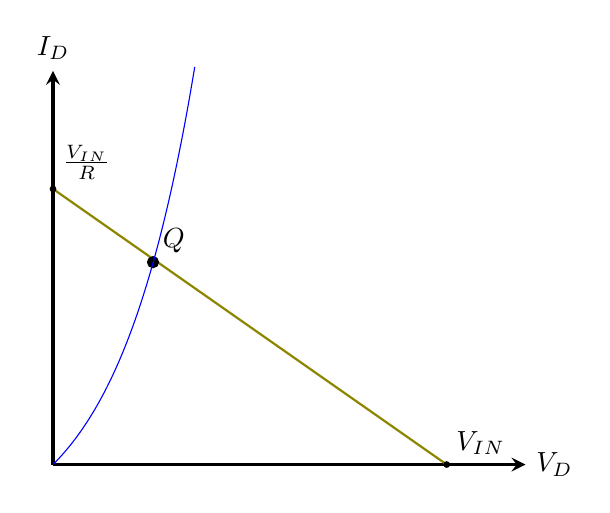
\begin{tikzpicture}[axis/.style={very thick, ->, >=stealth}]
    \draw[axis] (0,0) -- (6,0) node(xline)[right] {$V_D$};
    \draw[axis] (0,0) -- (0,5) node(yline)[above] {$I_D$};
    \draw[olive,thick] (0,3.5) -- (5,0);
    \filldraw [black]
    (1.27,2.57) circle (2pt) node[above right, black] {$Q$};
    \draw[scale=1,domain=0:1.8,smooth,variable=\x,blue] plot ({\x},{e^\x-1});
    \filldraw [black]
    (5, 0) circle (1pt) node[above right, black] {$V_{IN}$};
    \filldraw [black]
    (0, 3.5) circle (1pt) node[above right, black] {$\frac{V_{IN}}{R}$};
  \end{tikzpicture}
  \caption{}
  \label{grafico_1}
\end{figure}

Si può ora notare che la retta e la curva del diodo si intersecano in un unico punto Q, che rappresenta il punto dal quale il circuito "funziona". Possiamo ora ricavare dal grafico le coordinate di Q, che rappresentano rispettivamente la tensione e la corrente cercate e dunque la nostra soluzione.

\textbf{3. Linearizzazione a tratti}

Possiamo considerare il diodo con il suo modello ideale (Modello 0) e "linearizzare" così il circuito. Esistono ora due casi possibili: diodo ON  e diodo OFF. Poiché stiamo approssimando il diodo a un diodo ideale, nel caso ON potremo sostituirlo con un generatore di tensione da 0.7 Volt, mentre nel caso OFF lo sostituiremo con un circuito aperto.

Diodo ON:
\begin{center}
  \begin{circuitikz}
    \draw (0,4)
    to[american voltage source, v^<= $V_{IN}$]
    (0,0) node[ground] {};
    \draw (0,4)
    to[resistor = R, i=$I_D$,] (4,4)
    to[american voltage source, v<=$V{=0.7}$ ] node[ground] {} (4,0)
    ;\end{circuitikz}
\end{center}


Diodo OFF:
\begin{center}
  \begin{circuitikz}
    \draw (0,4)
    to[american voltage source, v^<= $V_{IN}$]
    (0,0) node[ground] {};
    \draw (0,4)
    to[resistor = R, i^>=$I{=0}$] (3,4) to[short, o-] (3,4);
  \end{circuitikz}
\end{center}


Alimentiamo il circuito preso in esame precedentemente e analizziamo i due casi.

Diodo ON:
\begin{center}
  \begin{circuitikz}
    \draw (4,8)
    node[above] {$V_{DD}{=5V}$} (4,8)
    node[tground] {} (4,8)
    to[american voltage source, v<=$V{=0.7}$ ](4,4)
    to[resistor = R, i=$I_D$,] (0,4)
    to[american voltage source, v^<= $V_{IN}$] (0,0)
    node[ground] {};
  \end{circuitikz}
\end{center}

\[I_D = \frac{V_{IN}-(5V+0.7V)}{R}\]
Se il diodo è ON, $I_D$ deve essere >0, $\Rightarrow$ $V_{IN}>5.7V$
Quindi il diodo è acceso per valori di $V_{IN}$ che siano maggiori di 5.7 V

Diodo OFF:
\begin{center}
  \begin{circuitikz}
    \draw (0,4)
    to[american voltage source, v^<= $V_{IN}$]
    (0,0) node[ground] {};
    \draw (0,4)
    to[resistor = R, i=$I_D$,] (4,4)
    to[short, *-o] (4,5.5)
    to[open] (4,6.5)
    to[short, o-] (4,8)
    node[above] {$V_{DD}{=5V}$} (4,8)
    node[tground] {} (4,8)
    (4,4) to[short, -o] (6,4) {} node[right] {$V_{OUT}=V_{IN}$}
    ;\end{circuitikz}
\end{center}

Per 0<$V_{IN}$<5.7 il diodo è OFF.

Dopo aver studiato i due casi, possiamo guardare la $V_{IN}$ data dal testo dell'esercizio che ci interessa risolvere, vedere in quale dei due casi cade e risolvere il circuito lineare del caso di nostro interesse.

\section{Raddrizzatori di tensione}
I diodi possono essere utilizzati per realizzare un raddrizzatore di tensione, ovvero convertire una tensione alternata in una tensione continua.
Quando consideriamo un alimentatore che fornisce tensione alternata, ci interessa sapere il suo valore efficace. Esso viene calcolato con la seguente formula:
\[V_{eff} = \frac{V_{Picco}}{\sqrt{2}}\]
Componente necessario per il raddrizzatore di tensione, insieme al diodo, è il trasformatore.
Il trasformatore è una macchina elettrica, composta da due avvolgimenti di spire su un nucleo:
\begin{figure}[H]
  \begin{center}
    \begin{circuitikz} \draw
      (0,0) node[transformer]{}
      ;\end{circuitikz}
  \end{center}
  \caption{Un trasformatore}
\end{figure}
Essendo $V_1$ e $V_2$ le tensioni sui due avvolgimenti, $n_1$ e $n_2$ i rispettivi numeri di spire, l'equazione del trasformatore è \[ \frac{V_{1}}{n_1}= \frac{V_{2}}{n_2}\]
Consideriamo un trasformatore collegato ad alimentazione, con l'alimentatore che lavora in regime sinusoidale.
La tensione trasmessa dal trasformatore è a sua volta sinusoidale:

\begin{figure}[H]
  \center
  \begin{tikzpicture}[axis/.style={very thick, ->, >=stealth}]
    \draw[axis] (0,0) -- (6,0) node(xline)[right] {$t$};
    \draw[axis] (0,-3) -- (0,3) node(yline)[above] {$V_D$};
    \draw plot[scale=0.5, domain=0:4*pi,smooth] (\x,{sin(\x r)});
  \end{tikzpicture}
  \caption{Tensione sinusoidale}
  \label{grafico_1}
\end{figure}

\subsection{Un semplice raddrizzatore di tensione}
Di seguito mostriamo la struttura di un semplice raddrizzatore:


\begin{figure}[H]
  \begin{center}
    \begin{circuitikz} \draw
      (0,0) node[transformer core]{} (1,0)
      (1,0) to[empty diode, i=$I$] (3,0)
      (3,0) to[capacitor = C](3,-2.1)
      (3,0) to[short, *-] (5,0)
      (5,0) to[resistor = R] (5,-2.1)
      (5,-2.1) to[short, -*](3,-2.1) -- (1,-2.1)
      ;\end{circuitikz}
  \end{center}
  \caption{Un semplice raddrizzatore di tensione}
\end{figure}

Quando il circuito della \textbf{figura 4} viene alimentato, $V_{OUT}$ raggiunga il valore $V_{Picco}-V{ON}$ quando l'ingresso raggiunge il valore di picco. Nel mentre il condensatore si carica.
Quando l'ingresso comincia a diminuire, il diodo si spegne e il condensatore inizia a scaricarsi.
Quando $V_{IN}-V{OUT}$ torna ad essere maggiore di $V_{ON}$, il diodo torna ON e il condensatore ricomincia a caricarsi.

\begin{center}
  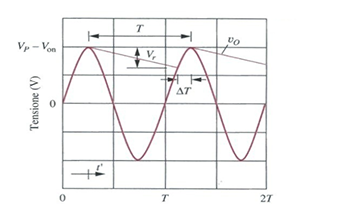
\includegraphics{raddrizzatore}
\end{center}

\subsection{Altri raddrizzatori di tensione}

Funzionano in modo analogo fra loro il raddrizzatore a ponte e il raddrizzatore a doppia semi-onda.

\begin{figure}[H]
  \begin{center}
    \begin{circuitikz}
      \draw(0,1) node[transformer core] {} ;

      \draw(1,1) to[empty diode] (2,2);
      \draw(2,2) to[empty diode] (3,1);
      \draw(1,1) to[empty diode] (2,0);
      \draw(2,0) to[empty diode] (3,1);

      \draw(1,1) to[short, *-] (1,1);
      \draw(3,1) to[short, *-] (3,-1.1) -- (1,-1.1);

      \draw(2,2) to[short, *-] (7,2);
      \draw(2,0) to[short, *-] (2,-0.5) -- (7,-0.5);

      \draw(5,2) to[short, *-] (5,2);
      \draw(5,2) to[capacitor = C] (5,-0.5);
      \draw(5,-0.5) to[short, *-] (5,-0.5);

      \draw(7,2) to[resistor  = R] (7,-0.5);

    \end{circuitikz}
  \end{center}
  \caption{Un raddrizzatore a ponte}
\end{figure}


\begin{figure}[H]
  \begin{center}
    \begin{circuitikz} \draw
      (0,0) node[transformer core]{} (1,0)
      (1,0) to[empty diode, i=$I$] (3,0)
      (3,0) to[capacitor = C](3,-2.1)
      (3,0) to[short, *-] (5,0)
      (5,0) to[resistor = R] (5,-2.1)
      (5,-2.1) to[short, -*] (3,-2.1)
      (1,-2.1) to[empty diode] (3,-2.1)
      ;\end{circuitikz}
  \end{center}
  \caption{Un raddrizzatore a doppia semi-onda}
\end{figure}

Per entrambi i raddrizzatori, vale:
\[V_{OUT} = (V_{IN}-1.4)\]
\[I_D = I_C + I_R= \frac{\partial{V_C}}{\partial{t}} - \frac{V_{OUT}}{R} \]

La differenza fra questi raddrizzatori e il raddrizzatore semplice visto precedentemente è che la distanza fra un'accensione del diodo e la successiva si riduce: nel raddrizzatore semplice trascorre un tempo uguale al periodo della sinusoide, con il raddrizzatore a doppia semi-onda e a ponte trascorre un tempo pare a metà periodo della sinusoide.

\begin{center}
  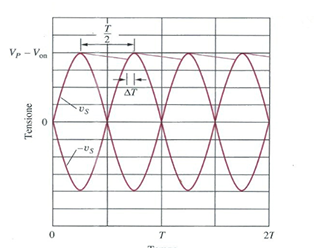
\includegraphics{raddrizzatore2}
\end{center}


\section{Come Risolvere gli esercizi sui diodi}
\subsection{Esercizio 5.1a}
Consideriamo il seguente circuito:

\begin{center}
  \begin{circuitikz}
    \draw (0,5.5) node[above] {$V_{dd}$} (0,5.5) node[tground] {} (0,5.5)
    (0,5.5) to[resistor=$R_1$] (0,2.5)
    (0,2.5) to[resistor=$R_2$] (0,0)
    (0,0) node[ground] {};
    \draw (0,2.5) to[short, *-o] (3,2.5) node[above] {$V_{out}$}
    (2,2.7) node[right] {A}
    (2,2.5) to[short, *-] (2,0) node[ground] {} (2,0) to[diode=$D_1$,v<=$V_{D}$ ](2,2);
  \end{circuitikz}
\end{center}


\begin{center}
  $V_{DD}=5V$

  $V_{SS}=1V$

  $R_1=2k\Omega$

  $R_2=3k\Omega$

\end{center}

\paragraph{(a)} Studiare lo stato di polarizzazione del diodo \paragraph{(b)} Ricavare $V_{OUT}$.


\subsection{Soluzione Esercizio 5.1a}
Solitamente questi circuiti vengono risolti facendo una supposizione iniziale sullo stato di funzionamento e verificando se questa porta a una condizione di assurdo. Se questo accade, l'ipotesi va scartata, altrimenti la accettiamo come valida.

\paragraph{(a)}
Supponiamo che il diodo sia ON.
Se il diodo è ON allora $V_D$ deve essere 0.7 V.
Supponiamo dunque $V_D=0.7 V$ e calcoliamo le correnti che scorrono nel circuito.

\[I_{R1} = \frac{V_{R1}}{R_1} = \frac{5V - (-0.7V)}{2k\Omega} = 2.85mA\]
\[I_{R2} = \frac{V_{R2}}{R_2} = \frac{0V - (-0.7V)}{3k\Omega} = 0.3mA\]

Applicando la legge di Kirchhoff al nodo si ottiene che nel diodo scorre una corrente \[I_{D} = I_{R1}+I_{R2} = 3.15mA\] positiva nel verso evidenziato nella figura sottostante:

CONTROLLARE I SEGNI E I VERSI DELLE CORRENTI!!!!

\begin{center}
  \begin{circuitikz}
    \draw (0,5.5) node[above] {$V_{dd}$} (0,5.5) node[tground] {} (0,5.5)
    (0,5.5) to[resistor=$R_1$, i>=$I_{R1}$] (0,2.5)
    (0,2.5) to[resistor=$R_2$, i<=$I_{R2}$] (0,0)
    (0,0) node[ground] {};
    \draw (0,2.5) to[short, *-o] (3,2.5) node[above] {$V_{out}$}
    (2,2.5) to[short, *-] (2,0) node[ground] {}
    (2,2.7) node[right] {A}
    (2,2)to[short, i>=$I_D$] (2, 1.4)
    (2,0) to[diode=$D_1$,v<=$V_{D}$ ](2,1.4);
  \end{circuitikz}
\end{center}

Questo è assurdo: in un diodo, se scorre corrente, non può scorrere in quel verso ma soltanto nel verso opposto.
Dunque il diodo non può essere acceso. Ci aspettiamo quindi che $V_{OUT}$ sia una tensione "piccola" (o negativa). 


\paragraph{(b)} Vogliamo ora calcolare $V_{OUT}$. Per farlo possiamo applicare il partitore di tensione:
\[V_{OUT} = V_{DD}\frac{R_2}{R_1+R_2} = 3V\]
Quindi $V_D=-3V$. 
Questo verifica l'ipotesi per cui il diodo debba essere OFF.



\subsection{Esercizio 5.1b}
\begin{center}
  \begin{circuitikz}
    \draw (0,5.5) node[above] {$V_{dd}$} (0,5.5) node[tground] {} (0,5.5)
    (0,5.5) to[resistor=$R_1$] (0,2.5)
    (0,2.5) to[resistor=$R_2$] (0,0)
    (0,0) node[ground] {};
    \draw (0,2.5) to[resistor=$R_3$, *-o] (2,2.5)
    (2,2.7) node[right] {A}
    (0,2.5) node[left] {$V_x$}
    (2,2.5) to[short, *-] (3,2.5) node[above] {$V_{out}$}
    (2,2.5) to[short, *-] (2,2) to[diode=$D_1$,v<=$V_{D}$ ](2,0) node[below] {$V_{ss}$};
  \end{circuitikz}
\end{center}

\begin{center}
  $V_{DD}=5V$

  $V_{SS}=1V$

  $R_1=2k\Omega$

  $R_2=3k\Omega$

  $R_3=1k\Omega$

\end{center}

\paragraph{(a)} Studiare lo stato di polarizzazione del diodo \paragraph{(b)} Ricavare $V_{OUT}$ e $V_x$.

\subsection{Soluzione Esercizio 5.1b}
\paragraph{(a)}
Procediamo in modo analogo all'esercizio precedente.
Supponiamo però, stavolta, che il diodo sia spento.
Se il diodo è spento \[I_{R1}=I_D=0\].
Applichiamo il partitore di tensione:
\[V_{X} = V_{DD}\frac{R_2}{R_1+R_2} = 3V\].
La caduta di tensione ai capi del diodo è 2V, che è \textbf{maggiore} di 0.7V.
Questo significa che il diodo \textbf{non} può essere spento.
Dobbiamo scartare l'ipotesi del diodo OFF.

\paragraph{(b)}
Prendiamo quindi il caso diodo ON e cerchiamo $V_x$.
Se il diodo è ON $V_{OUT}=0.7V$.
Applichiamo la legge di Kirchhoff al nodo A. Ne segue: $I_{R1}+I_{R2}+I_{R3}=0$.
Applico la legge di Ohm per ricavare le correnti in funzione di $V_x$.
Ricavo:
\[\frac{V_x-5V}{R_1} + \frac{V_x}{R_2} + \frac{V_x-0.7V}{R_3} =0 \]
Svolgendo i calcoli ottengo \[V_x = \frac{5V}{2k\Omega} + \frac{0.7V}{k\Omega} \]
da cui \[V_x=1.49V\].

\subsection{Esercizio 5.2}
Dato il circuito sottostante, determinarne la polarizzazione:

\begin{center}
  \begin{circuitikz}
    \draw (0,5.5) node[above] {$V_{dd}$} (0,5.5) node[tground] {}
    (0,5.5) to[resistor=$R_1$] (0,2.5)
    (0,2.5) to[diode] (0,0)
    (0,0) to[resistor=$R_2$] (0,-2)
    (0,-2) node[below] {$V_{ss1}$}
    (0,-2) node[tground] {};
    \draw (0,2.5) to[short, *-o] (3,2.5) node[above] {$V_{out}$}
    (2,2.5) to[short, *-] (2,2.3)
    (2,-2) node[below] {$V_{ss2}$} {}
    (2,-2) node[tground] {}
    (2,2.3) to[resistor=$R_4$] (2,0)
    (2,-2) to[diode=$D_1$,v<=$V_{D}$ ](2,0);
    \draw (2,6.5) node[above] {$V_{dd}$} (2,6.5) node[tground] {}
    (2,4.5) to[diode] (2,6.5)
    (2,4.5) to[resistor] (2,2.5)
    ;
  \end{circuitikz}
\end{center}

\begin{center}
  $V_{DD}=3V$

  $V_{ss1}=-2V$

  $V_{ss2}=-7V$

  $R_1=1k\Omega$

  $R_2=1.7k\Omega$

  $R_3=4.3k\Omega$

  $R_4=5k\Omega$

\end{center}




\end{document}